\section{Теоретичні відомості}
\subsection{Метод головних компонент}
Метод головних компонент (Principal component analysis) --- метод, що дозволяє
зменшити розмірність досліджуваної вибірки з мінімальними втратами інформації.
\cite{Aivazyan:1989}

Маємо $m$ об’єктів, з яких треба зняти по $n$ певних властивостей.
На вході в нас є виборки $\vec{X}_k$, кожна з яких відповідає сукупності
властивостей $k$-го об’єкту
\begin{equation*}
  \vec{X}_k = \begin{bmatrix}
    x_k^1  \\
    x_k^2  \\
    \vdots \\
    x_k^n
  \end{bmatrix},
  \qquad k = \overline{1,m}
\end{equation*}
Згрупуємо всі вимірювання в одну матрицю $X$
\begin{equation*}
  X = \begin{bmatrix}
    x_1^1  & x_2^1  & \dots  & x_m^1  \\
    x_1^2  & x_2^2  & \dots  & x_m^2  \\
    \vdots & \vdots & \ddots & \vdots \\
    x_1^n  & x_2^n  & \dots  & x_m^n
  \end{bmatrix}
\end{equation*}

Спочатку нам знадобиться знайти вибіркові середні значення для кожної
властивості
\begin{equation*}
  a_i = \frac{1}{m} \cdot \sum_{k=1}^{m} x_k^i, \qquad i = \overline{1,n}
\end{equation*}
Маємо вектор вибіркових середніх значень
\begin{comment}
\begin{equation*}
  \vec{a} = \begin{bmatrix}
    \frac{1}{m} \sum_{k=1}^{m} x_k^1 \\
    \frac{1}{m} \sum_{k=1}^{m} x_k^2 \\
    \vdots                           \\
    \frac{1}{m} \sum_{k=1}^{m} x_k^n \\
  \end{bmatrix}
\end{equation*}
\end{comment}
\begin{equation*}
  \vec{a} = \begin{bmatrix}
    a_1    \\
    a_2    \\
    \vdots \\
    a_n
  \end{bmatrix}
\end{equation*}

Центруємо отримані дані, що містяться в матриці $X$, віднявши від кожного
стовбця вектор вибіркових середніх $\vec{a}$
\begin{comment}
\begin{equation*}
  \tilde{x}_k^i = x_k^i - a_i,\qquad k = \overline{1,m}, i = \overline{1,n}
\end{equation*}
Кожен стовбець матриці вимірювань прийме вигляд
\begin{equation*}
  \tilde{X}_k
  = \vec{X}_k - \vec{a}
  = \begin{bmatrix}
    x_k^1 - a_1 \\
    x_k^2 - a_2 \\
    \vdots      \\
    x_k^n - a_n
  \end{bmatrix},
  \qquad k = \overline{1,m}
\end{equation*}
Маємо матрицю центрованих вимірювань $\tilde{X}$
\end{comment}
\begin{equation*}
  \tilde{X}
  = \begin{bmatrix}
    \tilde{x}_1^1  & \tilde{x}_2^1  & \dots  & \tilde{x}_m^1  \\
    \tilde{x}_1^2  & \tilde{x}_2^2  & \dots  & \tilde{x}_m^2  \\
    \vdots & \vdots & \ddots & \vdots \\
    \tilde{x}_1^n  & \tilde{x}_2^n  & \dots  & \tilde{x}_m^n
  \end{bmatrix}
  = \begin{bmatrix}
    x_1^1 - a_1  & x_2^1 - a_1  & \dots  & x_m^1 - a_1 \\
    x_1^2 - a_2  & x_2^2 - a_2  & \dots  & x_m^2 - a_2 \\
    \vdots       & \vdots       & \ddots & \vdots      \\
    x_1^n - a_n  & x_2^n - a_n  & \dots  & x_m^n - a_n
  \end{bmatrix}
\end{equation*}

Обчислюємо вибіркову коваріаційну матрицю властивостей.
Вибіркову коваріацію $i$ та $j$ властивості рахуємо за формулою
\begin{equation*}
  \sigma_i^j
  = \frac{1}{m} \cdot \sum_{k=1}^{m} \tilde{x}_k^i \cdot \tilde{x}_k^j
  = \frac{1}{m} \cdot \sum_{k=1}^{m}
    \left[ \left( x_k^i - a_i \right) \cdot \left( x_k^j - a_j \right) \right],
    \qquad i,j = \overline{1,n}
\end{equation*}
Маємо вибіркову коваріаційну матрицю
\begin{equation*}
  K = \begin{bmatrix}
    \sigma_1^1 & \sigma_2^1 & \dots  & \sigma_n^1 \\
    \sigma_1^2 & \sigma_2^2 & \dots  & \sigma_n^2 \\
    \vdots     & \vdots     & \ddots & \vdots     \\
    \sigma_1^n & \sigma_2^n & \dots  & \sigma_n^n \\
  \end{bmatrix}
\end{equation*}
\begin{comment}
\begin{equation*}
  K =
  \begin{bmatrix}
    \frac{1}{m} \cdot \sum_{k=1}^{m} \tilde{x}_k^1 \cdot \tilde{x}_k^1
    &
    \frac{1}{m} \cdot \sum_{k=1}^{m} \tilde{x}_k^1 \cdot \tilde{x}_k^2
    &
    \dots
    &
    \frac{1}{m} \cdot \sum_{k=1}^{m} \tilde{x}_k^1 \cdot \tilde{x}_k^n
    \\
    \frac{1}{m} \cdot \sum_{k=1}^{m} \tilde{x}_k^2 \cdot \tilde{x}_k^1
    &
    \frac{1}{m} \cdot \sum_{k=1}^{m} \tilde{x}_k^2 \cdot \tilde{x}_k^2
    &
    \dots
    &
    \frac{1}{m} \cdot \sum_{k=1}^{m} \tilde{x}_k^2 \cdot \tilde{x}_k^n
    \\
    \vdots & \vdots & \dots & \vdots \\
    \frac{1}{m} \cdot \sum_{k=1}^{m} \tilde{x}_k^n \cdot \tilde{x}_k^1
    &
    \frac{1}{m} \cdot \sum_{k=1}^{m} \tilde{x}_k^n \cdot \tilde{x}_k^2
    &
    \dots
    &
    \frac{1}{m} \cdot \sum_{k=1}^{m} \tilde{x}_k^n \cdot \tilde{x}_k^n
  \end{bmatrix}
\end{equation*}
\end{comment}

Щоб отримувати лише потрібну інформацію, ми хочемо знайти таке ортогональне
лінійне перетворення $L$ вхідної матриці $\tilde{X}$, щоб отримати матрицю
$Y = L \cdot \tilde{X}$, яка має діагональну вибіркову ковариаційну матрицю $K'$
з незростаючими зверху вниз значеннями.
Діагональна вибіркова коваріаційна матриця гарантує той факт, що отримані
значення $Y$ будуть некорельованими.
Рангування значень діагональних елементів матриці $K'$ за величиною дасть більш
наочне уявлення про будову досліджуваних об’єктів, адже діагональні
елементи --- вибіркові дисперсії.
Чим більше дисперсія, тим більше відповідна властивість змінюється від об’єкту
до об’єкту, і тим більше корисної інформації вона нам надає.

Вибіркова коваріаційна матриця $K'$ для $Y = L \cdot \tilde{X}$ має вигляд
\begin{equation*}
  K'
  = L \cdot K \cdot L^*
  = \begin{bmatrix}
    \lambda_1 & 0         & \dots  & 0      \\
    0         & \lambda_2 & \dots  & 0      \\
    \vdots    & \vdots    & \ddots & \vdots \\
    0         & 0         & \dots  & \lambda_n
  \end{bmatrix}
\end{equation*}
З лінійної алгебри відомо, що матриця $L$ складається з координат власних
векторів матриці $K$, а елементи $\lambda_k$ --- її власні числа, які
існують і є невід’ємними через невід’ємну означеність матриці $K$.
Вважаємо, що числа $\lambda_1, \dots, \lambda_n$ впорядковані від більшого до
меншого для зручності подальших дій.
Позначимо власний вектор матриці $K$, що відповідає власному числу $\lambda_k$,
як $\vec{l}_k$. Тоді
\begin{equation*}
  \vec{l}_k
  = \left[ l_k^1, l_k^2, \dots, l_k^n \right],
  \qquad k = \overline{1,n}
\end{equation*}
Матриця $L$ має вигляд
\begin{equation*}
  L = \begin{bmatrix}
    l_1^1  & l_1^2  & \dots  & l_1^n  \\
    l_2^1  & l_2^2  & \dots  & l_2^n  \\
    \vdots & \vdots & \ddots & \vdots \\
    l_n^1  & l_n^2  & \dots  & l_n^n  \\
  \end{bmatrix}
\end{equation*}

Треба зменшити розмірність простору досліджуваних параметрів системи з $n$ до
$p<n$, але при цьому втратити якомога менше відомостей про досліджувані
об’єкти.
Введемо міру інформації, що залишається при зменшенні кількості компонент, що
розглядаються
\begin{equation*}
  I = \frac{\lambda_1 + \dots + \lambda_p}{\lambda_1 + \dots + \lambda_n}
\end{equation*}
Будемо вважати, що діємо продуктивно, тому починаємо обирати з перших
компонент, адже саме вони є найбільш інформативними.
Також бачимо, що інформативність змінюється в межах від $0$
(нічого не дізнаємось) до $1$ (зберегли усю інформацію).

Надалі буде розглядатися матриця головних компонент $Y$
\begin{equation*}
  Y = \begin{bmatrix}
    y_1^1  & y_2^1  & \dots  & y_m^1  \\
    y_1^2  & y_2^2  & \dots  & y_m^2  \\
    \vdots & \vdots & \ddots & \vdots \\
    y_1^p  & y_2^p  & \dots  & y_m^p  \\
    \end{bmatrix}
\end{equation*}
\subsection{Гістограма}

Для подальшого аналізу потрібно здобути щільність розподілу головних компонент.
Оскільки маємо справу з вибіркою і вибірковими характеристиками,
потрібно побудувати гістограму, адже це і є вибіркова характеристика,
що відповідає щільності.

Побудуємо $j$-й стовбець гістограми для виборки з $k$-ї строки матриці $Y$
\begin{equation*}
  h_j^k = \frac{1}{m} \cdot \sum_{i=1}^{m} \indicator{y_i^k \in I_j^k},
  \qquad j = \overline{1, N},
  \qquad k = \overline{1, p}
\end{equation*}
де $I^k$ --- набір напівінтервалів, що розбиває відрізок
$\left[ \min\limits_{i=\overline{1,m}}{y_i^k};
\max\limits_{i=\overline{1,m}}{y_i^k} \right]$ на $N$ рівних частин.
Для вибору $N$ можна скористатися досить відомою формулою Стьорджеса
(Sturges' formula) \cite{Sturges:1926:CCI}
\begin{equation*}
  N = \lfloor \log_2 m \rfloor + 1
\end{equation*}
Маємо матрицю гістограм
\begin{equation*}
  H = \begin{bmatrix}
    h_1^1  & h_2^1  & \dots  & h_N^1  \\
    h_1^2  & h_2^2  & \dots  & h_N^2  \\
    \vdots & \vdots & \ddots & \vdots \\
    h_1^p  & h_2^p  & \dots  & h_N^p
  \end{bmatrix}
\end{equation*}
і напівінтервалів, що відповідають кожному стовбчику кожної гістограми
\begin{equation*}
  I = \begin{bmatrix}
    I_1^1  & I_2^1  & \dots  & I_N^1  \\
    I_1^2  & I_2^2  & \dots  & I_N^2  \\
    \vdots & \vdots & \ddots & \vdots \\
    I_1^p  & I_2^p  & \dots  & I_N^p
  \end{bmatrix}
\end{equation*}

\subsection{Критерій узгодженості Пірсона $\chi^2$}
Гістограма може використовуватися не тільки для графічної інтерпретації
отриманих даних, але й для віднесення вибірки до якогось відомого розподілу.
Відповідь на питання ``Чи дійсно вибірка $y_1^k$, $\dots$, $y_m^k$ має розподіл
$F^k$?'' може надати критерій узгодженості Пірсона.

Розглянемо вектор
\begin{equation*}
    \eta^k
    = \left[ \frac{\nu_1^k - m \cdot \rho_1^k}{\sqrt{m \cdot \rho_1^k}}, \dots,
      \frac{\nu_N^k - m \cdot \rho_N^k}{\sqrt{m \cdot \rho_N^k}} \right]
\end{equation*}
Знайдемо його характеристичну функцію
\begin{equation*}
  \varphi_{\eta^k}\left( \lambda\right)
  = \mean{e^{i \cdot \left( \lambda, \eta^k \right)}},\qquad
  \lambda \in \mathbb{R}^N
\end{equation*}
Для зручності перепозначимо індикатор
\begin{equation*}
  \mathfrak{I}_{i,j}^k = \Indicator{y_i^k \in I_j^k}
\end{equation*}
Подивимось, чому дорівнює скалярний добуток в експоненті
\begin{equation*}
  \begin{split}
    \left( \lambda, \eta^k \right)
    &= \sum_{j=1}^{N} \lambda_j \cdot \frac{\nu_j^k - m \cdot \rho_j^k}{
      \sqrt{m \cdot \rho_j^k}}
    = \sum_{j=1}^{N}\frac{\lambda_j}{\sqrt{m \cdot \rho_j^k}}
      \cdot \sum_{i=1}^{m}\left( \mathfrak{I}_{i,j}^k - \rho_j^k \right) = \\
    &= \sum_{j=1}^{N} \sum_{i=1}^{m}
      \frac{\lambda_j}{\sqrt{m \cdot \rho_j^k}}
      \cdot \left( \mathfrak{I}_{i,j}^k - \rho_j^k \right)
    = \sum_{i=1}^{m} \sum_{j=1}^{N} \lambda_j \cdot
      \frac{\mathfrak{I}_{i,j}^k - \rho_j^k}{\sqrt{m \cdot \rho_j^k}}
  \end{split}
\end{equation*}
Бачимо суму $m$ незалежних однаково розподілених випадкових величин.
Введемо позначення
\begin{equation*}
  \mathfrak{I}_j^k = \Indicator{y_1^k \in I_j^k}
\end{equation*}
А також позначимо новий випадковий вектор
\begin{equation*}
  \zeta^k
  = \left[ \frac{\mathfrak{I}_1^k - \rho_1^k}{\sqrt{m \cdot \rho_1^k}},
    \dots
    \frac{\mathfrak{I}_N^k - \rho_N^k}{\sqrt{m \cdot \rho_N^k}} \right]
\end{equation*}
Тоді скалярний добуток прийме вигляд
\begin{equation*}
    \left( \lambda, \eta^k \right)
    = \sum_{i=1}^{m} \sum_{j=1}^{N} \lambda_j \cdot \zeta_j^k
    = \sum_{i=1}^{m} \left( \lambda, \zeta^k \right)
    = m \cdot \left( \lambda, \zeta^k \right)
\end{equation*}
За рахунок незалежності випадкових величин $\zeta_j^k$ маємо
\begin{equation}\label{eq:cf:eta}
  \varphi_{\eta^k}\left( \lambda\right)
  = \mean{e^{i \cdot \left( \lambda, \eta^k \right)}}
  = \mean{e^{m \cdot i \cdot \left( \lambda, \zeta^k \right)}}
  = \left( \mean{e^{i \cdot \left( \lambda, \zeta^k \right)}} \right)^m
\end{equation}
Розглянемо характеристичну функцію випадкового вектора $\zeta^k$
\begin{equation}\label{eq:cf:zeta}
  \varphi_{\zeta^k}\left( \lambda \right)
  = \Mean{\exp{\left\{ i
    \cdot \sum_{j=1}^{N} \lambda_j \cdot \zeta_j^k \right\}}}
\end{equation}
Легко побачити, що
\begin{equation*}
  \begin{split}
    \left( \lambda, \zeta^k \right)
    = \sum_{j=1}^{N} \lambda_j \cdot \zeta_j^k
    = \sum_{j=1}^{N} \lambda_j
      \cdot \frac{\mathfrak{I}_j^k - \rho_j^k}{\sqrt{m \cdot \rho_j^k}}
    &= \sum_{j=1}^{N} \left(
       \frac{\lambda_j}{\sqrt{m \cdot \rho_j^k}} \cdot \mathfrak{I}_j^k
       - \frac{\sqrt{\rho_j^k} \cdot \lambda_j}{\sqrt{m}} \right) = \\
    &= \sum_{j=1}^{N} \mathfrak{I}_j^k \cdot \left( 
        \frac{\lambda_j}{\sqrt{m \cdot \rho_j^k}}
        - \sum_{l=1}^{N} \frac{\sqrt{\rho_l^k} \cdot \lambda_l}{\sqrt{m}}
      \right)
  \end{split}
\end{equation*}
Тобто характеристична функція \eqref{eq:cf:zeta} приймає вигляд
\begin{equation*}
  \varphi_{\zeta^k}\left( \lambda \right)
  = \Mean{\sum_{j=1}^{N} \mathfrak{I}_j^k
    \cdot \exp{\left\{ \frac{i}{\sqrt{m}} \left(
      \frac{\lambda_j}{\sqrt{\rho_j^k}}
      - \sum_{l=1}^{N} \sqrt{\rho_l^k} \cdot \lambda_l \right) \right\}}}
\end{equation*}
Перепозначимо вираз в круглих дужках
\begin{equation*}
  \mathfrak{z}^k
  = \frac{\lambda_j}{\sqrt{\rho_j^k}}
    - \sum_{l=1}^{N} \sqrt{\rho_l^k} \cdot \lambda_l
\end{equation*}
Математичне очікування індикатора --- ймовірність події, яку він перевіряє.
Отже
\begin{equation*}
  \varphi_{\zeta^k}\left( \lambda \right)
  = \sum_{j=1}^{N} \rho_j^k
    \cdot \exp{\left\{ \frac{i \cdot \mathfrak{z}^k}{\sqrt{m}} \right\}}
\end{equation*}

Якщо розмір вибірки $m$ буде зростати, то характеристична функція $\eta^k$
\eqref{eq:cf:eta} буде поводитись наступним чином
\begin{equation*}
  \begin{split}
    \lim_{m \to \infty} \varphi_{\eta^k}\left( \lambda \right)
    &= \lim_{m \to \infty} \left( 1 + \sum_{k=1}^{N} p_k \cdot \left[
      \exp{\left\{ \frac{i \cdot \mathfrak{z}^k}{\sqrt{m}} \right\}}
      - 1 \right] \cdot \frac{m}{m} \right)^m = \\
    &= \lim_{m \to \infty} \exp{ \left\{ m \cdot \sum_{k=1}^{N} p_k \cdot \left[
      \exp{\left\{ \frac{i \cdot \mathfrak{z}^k}{\sqrt{m}} \right\}}
      - 1 \right] \right\}}
  \end{split}
\end{equation*}
Для $\exp{\left\{ \frac{i \cdot \mathfrak{z}^k}{\sqrt{m}} \right\}}$
використаємо співвідношення
\begin{equation*}
  e^{\alpha} - 1 \approx \alpha + \frac{\alpha^2}{2},\qquad \alpha \ll 1
\end{equation*}
Маємо
\begin{equation*}
  \begin{split}
    \sum_{j=1}^{N} \rho_j^k \cdot \frac{i \cdot \mathfrak{z}^k}{\sqrt{m}}
    &= \sum_{j=1}^{N} \rho_j^k \cdot \frac{i}{\sqrt{m}}
      \cdot \left( \frac{\lambda_j}{\sqrt{\rho_j^k}}
        - \sum_{l=1}^{N} \sqrt{\rho_l^k} \cdot \lambda_l \right) = \\
    &= \frac{i}{\sqrt{m}} \cdot \left(
      \sum_{j=1}^{N} \sqrt{\rho_j^k} \cdot \lambda_j
      - \sum_{l=1}^{N} \sqrt{\rho_l^k} \cdot \lambda_l \right)
    = 0,
  \end{split}
\end{equation*}
\begin{equation*}
  \begin{split}
    \sum_{j=1}^{N} \rho_j^k
      \cdot \left( \frac{i \cdot \mathfrak{z}^k}{\sqrt{m}} \right)^2
      = - \sum_{j=1}^{N} \frac{\rho_j^k}{m}
        \cdot \left( \frac{\lambda_j}{\sqrt{\rho_j^k}}
          - \sum_{l=1}^{N} \sqrt{\rho_l^k} \cdot \lambda_l \right)^2 = \\
      = - \frac{1}{m} \cdot \left[ \sum_{j=1}^{N} \lambda_j
        - \left( \sum_{l=1}^{N} \sqrt{\rho_l^k} \cdot \lambda_l \right)^2
          \right]
  \end{split}
\end{equation*}
Тому
\begin{equation*}
  \begin{split}
    \lim_{m \to \infty} \varphi_{\eta^k}\left( \lambda \right)
    &= \lim_{m \to \infty} \exp{\left\{ -\frac{m}{m \cdot 2}
      \cdot \left[ \sum_{j=1}^{N} \lambda_j
        - \left( \sum_{l=1}^{N} \sqrt{\rho_l^k} \cdot \lambda_l \right)^2
        \right]\right\}} = \\
    &= \exp{\left\{ -\frac{1}{2} \cdot
      \left[ \sum_{j=1}^{N} \lambda_j
        - \left( \sum_{l=1}^{N} \sqrt{\rho_l^k} \cdot \lambda_l \right)^2
        \right] \right\}}
    = e^{-\frac{1}{2} \cdot \left( A^k \lambda, \lambda \right)}
  \end{split}
\end{equation*}
Матриця $A^k$ побудована наступним чином
\begin{equation*}
  A^k
  = \left\| \delta_{ij} - \sqrt{\rho_i^k} \cdot \sqrt{\rho_j^k} \right\|_{i=1}^n
\end{equation*}
Симетричність мариці очевидна, тому треба довести її невід’ємну визначеність,
щоб стверджувати, що вона є коваріаційною.
Для цього візьмемо вектор
\begin{equation*}
  e^k = \left[ \sqrt{\rho_1^k}, \dots, \sqrt{\rho_N^k} \right],\qquad
  \left\| e^k \right\| = 1
\end{equation*}
Тоді бачимо, що
\begin{equation}\label{eq:chi2:quadraticForm}
  \left( A^k \lambda, \lambda \right)
  = \left\| \lambda \right\|^2
    - \left( \lambda, e^k \right)^2
\end{equation}
З нерівності Коші маємо
\begin{equation*}
  \left\| \left( \lambda, e^k \right) \right\|
  \le \left\| \lambda \right\| \cdot \left\| e^k \right\|
  = \left\| \lambda \right\|
\end{equation*}
Тобто матриця є дійсно невід’ємно визначеною і вектор $\eta^k$ розподілений
за нормальним законом з нульовим середнім і коваріаційною матрицею $A^k$.

Для подальших розрахунків розглянемо стандартний гаусівський вектор
як суму випадкових нормально розподілених випадкових величин в стандартному
базисі $\mathbb{R}^N$, який позначимо $\left[ e_1, \dots, e_N \right]$
\begin{equation*}
  \xi = \sum_{j=1}^{N}\xi_j \cdot e_j \sim N\left( \vec{0}, I \right)
\end{equation*}
Згадуємо, що ортогональні перетворення $U$ зберігають відстані, а також
справедливо наступне
\begin{equation*}
  U\xi \sim N\left( 0, U I U^{-1} \right) \sim N\left( \vec{0}, I \right)
\end{equation*}
Також ортонормований базис залишається ортонормованим базисом після
ортогонального перетворення $U$.
Оберемо такий оператор $U$, щоб набір $\left[ e_1, \dots, e_N \right]$ під його
дією перетворився на $\left[ f_1, \dots, f_N \right]$, де
\begin{equation*}
  f_1 = e^k = \left[ \sqrt{\rho_1^k}, \dots, \sqrt{\rho_N^k} \right]
\end{equation*}
Тоді маємо вектор
\begin{equation*}
  U\xi
  = \hat{\xi}
  = \sum_{j=1}^{N} \hat{\xi_j} \cdot f_j \sim N\left( \vec{0}, I \right)
\end{equation*}
Подивимось, який розподіл має наступний вектор
\begin{equation*}
  \Upsilon
  = \sum_{j=2}^{N} \hat{\xi_j} \cdot f_j
  = \hat{\xi} - \hat{\xi_1} \cdot e^k
\end{equation*}
Для цього розглянемо квадратичну форму
\begin{equation*}
  \mean{\left( \Upsilon, \lambda \right)^2}
  = \sum_{j=2}^{N} \left( \lambda, f_j \right)^2
  = \sum_{j=1}^{N} \left( \lambda, f_j \right)^2 - \left( \lambda, f_1 \right)^2
  = \left\| \lambda \right\|^2 - \left( \lambda, e^k \right)^2
  = \left( A^k \lambda, \lambda \right)
\end{equation*}
З рівності \eqref{eq:chi2:quadraticForm} бачимо, що випадкові вектори $\eta^k$
та $\Upsilon$ мають однаковий розподіл.
Отже, розподіли їх норм теж співпадають.
Оскільки сума $N-1$ квадратів незалежних стандартних гаусових випадкових
величин має розподіл Пірсона з $N-1$ ступенями вільності
\begin{equation*}
  \left\| \Upsilon \right\|^2 = \sum_{j=2}^{N} \xi_j^2 \sim \chi_{N-1}^2
\end{equation*}
Маємо
\begin{equation*}
  \left\| \eta^k \right\|
  = \sum_{j=1}^{N}\frac{\left( \nu_j^k - m \cdot \rho_j^k \right)^2}{
    m \cdot \rho_j^k}
  = m \cdot \sum_{j=1}^{N}\frac{\left( h_j^k - \rho_j^k \right)^2}{\rho_j^k}
  \sim \chi_{N-1}^2
\end{equation*}

Останнє співвідношення дає змогу перевіряти належність виборки
$y_1^k$, $\dots$, $y_m^k$ до розподілу $F^k$.
Перевірка виглядає наступним чином.

Розглянемо випадкову величину
\begin{equation}\label{eq:pearson:Rk}
  R^k
  = m \cdot \sum_{j=1}^{N}\frac{\left( h_j^k - \rho_j^k \right)^2}{\rho_j^k}
\end{equation}

Обираємо рівень значущості $\alpha$ для функції розподілу $\chi_{N-1}^2$ і
шукаємо відповідне до кількості ступенів вільності $r_{\alpha}$.
Рівень значущості --- ймовірність помилки першого роду, тобто ймовірність того,
що буде відкинуто вірну гіпотезу
\begin{equation*}
  \probability{\chi_{N-1}^2 \ge r_{\alpha}} = \alpha
\end{equation*}
Якщо $R^k \le r_{\alpha}$, то гіпотеза про те, що вибірка $Y^k$ дійсно має
розподіл $F^k$, приймається.

Розглянемо той випадок, коли ймовірність $\rho_i^k$
відгадана невірно. Повернемося до формули \eqref{eq:pearson:Rk}
\begin{equation*}
  R^k
  = \sum_{j=1}^{N}\frac{\left( \nu_j^k - m \cdot \rho_j^k \right)^2}{m \cdot \rho_j^k}
\end{equation*}
Всі члени суми є невід’ємними. Якщо хоча б один елемент буде завеликим,
то великою буде вся сума. Маємо випадкову величину $\eta$
\begin{equation*}
  \eta
  = \nu_i^k - m \cdot \rho_i^k
  = \sum_{j=1}^{m} \left( \xi_j - \rho_i^k \right),
  \qquad \indicator{y_j^k \in I_i^k} = \xi_j
\end{equation*}
Якщо $\rho_i^k$ вгадано невірно, то воно не дорівнює математичному очікуванню
індикатора. Додамо та віднімемо справжнє математичне очікування
\begin{equation*}
  \eta
  = \sum_{j=1}^{m} \left( \xi_j - \mean{\xi_1} + \mean{\xi_1} - \rho_i^k \right)
  = \sum_{j=1}^{m} \left( \xi_j - \mean{\xi_1} \right)
    + \sum_{j=1}^{m} \left( \mean{\xi_1} - \rho_i^k \right)
\end{equation*}
Останній доданок є просто різницею, помноженою на $m$
\begin{equation*}
  \eta
  = \sum_{j=1}^{m} \left( \xi_j - \mean{\xi_1} \right)
    + m \cdot \left( \mean{\xi_1} - \rho_i^k \right)
\end{equation*}
Поділимо на $\sqrt{m}$, щоб скористатися центральною граничною теоремою
\begin{equation*}
  \frac{\eta}{\sqrt{m}}
  = \frac{1}{\sqrt{m}} \cdot \sum_{j=1}^{m} \left( \xi_j - \mean{\xi_1} \right)
    + \frac{1}{\sqrt{m}} \cdot m \cdot \left( \mean{\xi_1} - \rho_i^k \right)
\end{equation*}
Перший доданок асимптотично має розподіл $N\left( 0, \sigma^2 \right)$, де
$\sigma^2$ --- дисперсія випадкової величини $\xi_1$ для достатньо великих $m$.
Отже, вся сума зростає пропорційно до $\sqrt{m}$
\begin{equation*}
  \frac{\eta}{\sqrt{m}}
  = \frac{1}{\sqrt{m}} \cdot \sum_{j=1}^{m} \left( \xi_j - \mean{\xi_1} \right)
    + \sqrt{m} \cdot \left( \mean{\xi_1} - \rho_i^k \right)
  \sim \sqrt{m} \cdot \left( \mean{\xi_1} - \rho_i^k \right)
\end{equation*}
Тобто зараз $R^k$ буде зростати пропорційно до величини
$m$, і буде великим у порівнянні з $r_{\alpha}$, що призведе до відхилення
невірної гіпотези.

\subsection{Типи вищої нервової діяльності}

Для визначення того, які показники вимірювати і яким чином,
скористуємось відомою класифікацією типів вищої нервової діяльності.

Згідно з Павловим\cite{Pavlov:1923} типи вищої нервової діяльності
характеризуються трьома показниками: сила нервової системи (сильна або слабка),
врівноваженість (врівноважена або неврівноважена)
та рухливість (рухлива або інетртна).
Павлов розглядає 4 комбінації цих показників з 8 можливих:
\begin{enumerate}
  \item Слабка
  \item Сильна та неврівноважена
  \item Сильна, врівноважена та інертна
  \item Сильна, врівноважена та рухлива
\end{enumerate}
Далі ці класи (комбінації) будуть називатися відповідно слабкий,
неврівноважений, інертний та рухливий.
%Щоб віднести людину до того чи іншого класу, існує тест Айзенка.
%Складність полягає в тому, що не дуже часто зустрічаються чисті типи ---
%зазвичай вони змішані.

\subsection{Теппінг-тест (Tapping rate)}

Існують відомі залежності між типом вищої нервової діяльності та зміною
максимального темпу рухів кистю руки з часом.
Протягом 30 секунд людина намагається притримуватися максимально можливого для
себе темпу.
Показники темпу фіксуються через кожні 5 секунд, а далі по 6 отриманим точкам
будується крива темпа руху. \cite{Ilin:2001}

Для тесту можна використовувати ручку (олівець) і папір, або телеграф.
Сучасні технології дозволяють проводити тест за допомогою клавіатури комп’ютера
або екрану планшета.

З олівцем і папіром тест поводиться наступним чином:
\begin{enumerate}
  \item На папері креслиться 6 квадратів
  \item Людина починає ставити якомога більше точок в першому квадраті впродовж
    перших 5 секунд
  \item Коли проходить 5 секунд, потрібно перейти до наступного квадрату і
    ставити точки там
  \item Процедура повторюється до тих пір, доки не пройде 30 секунд --- в кінці
    буде заповнено всі 6 квадратів
\end{enumerate}
Далі підраховується кількість точок в кожному квадраті та малюється ламана, де
горизонтальна вісь відповідає номеру часового проміжку (номеру квадрата), а
вертикальна відповідає кількості точок в квадраті.

Трактуються отримані дані наступним чином:
\begin{enumerate}
  \item Спадна ламана відповідає слабкому типу (рис. \ref{fig:tapping:weak}).
    Вона спадає після перших 5 секунд тесту і не повертається до початкового
    рівня
  \item Ламана, що спочатку зростає, а після 10-15 секунд спадає нижче
    початкового рівня (проміжна між рівною та опуклою) відповідає
    неврівноваженому типу (рис. \ref{fig:tapping:middle}).
  \item Ввігнута ламана відповідає інертному типу
    (рис. \ref{fig:tapping:concave}).
    Вона спочатку спадає, а на 25-30 секундах може зрости до початкового темпу
  \item Опукла ламана відповідає рухливому типу
    (рис. \ref{fig:tapping:movable}).
    Це така ламана, що зростає в перші 10-15 секунд тесту, а після 25-30
    секунд повертається або падає нижче початкового рівня
  \item Також темп може залишатися приблизно на одному рівні протягом
    усього тесту, що є оптимальним для складання іспитів
    (рис. \ref{fig:tapping:flat}).
\end{enumerate}

Достовірним відхиленням достатньо вважати різницю в два і більше натиснення між
двома сусідніми п’ятисекундними проміжками. \cite{Ilin:2001}

Оскільки цей тест заснований на вимірюванні витривалості нервової системи людини
за умови максимального навантаження та перевіряє темп реагування (натиснення) на
подразнювачі (внутрішній подразнювач --- команда собі ``треба тиснути''),
було вирішено використовувати відомі вигляди кривих
(рис. \ref{fig:studentBehaviorSimple}) при моделюванні результатів
виконання завдань однакової складності.

\begin{figure}[h]
  \centering
  \begin{subfigure}[b]{0.3\textwidth}
  \resizebox{\textwidth}{!}{\drawHist{chartMovable}}
                \caption{Опукла}
                \label{fig:tapping:movable}
  \end{subfigure}
  \begin{subfigure}[b]{0.3\textwidth}
  \resizebox{\textwidth}{!}{\drawHist{chartMiddle}}
                \caption{Проміжна}
                \label{fig:tapping:middle}
  \end{subfigure}
  \begin{subfigure}[b]{0.3\textwidth}
  \resizebox{\textwidth}{!}{\drawHist{chartFlat}}
                \caption{Рівна}
                \label{fig:tapping:flat}
  \end{subfigure}\\[2ex]
  \begin{subfigure}[b]{0.3\textwidth}
  \resizebox{\textwidth}{!}{\drawHist{chartConcave}}
                \caption{Ввігнута}
                \label{fig:tapping:concave}
  \end{subfigure}
  \begin{subfigure}[b]{0.3\textwidth}
  \resizebox{\textwidth}{!}{\drawHist{chartWeak}}
                \caption{Спадна}
                \label{fig:tapping:weak}
  \end{subfigure}
  \caption{Загальний вигляд залежностей кількості поставлених точок від часу.
  Пунктирна лінія --- кількість точок в перші 5 секунд}
  \label{fig:studentBehaviorSimple}
\end{figure}

Потрібно зауважити, що швидкість розв’язування задач може змінюватися з
досвідом.
Тобто, якщо студент зі слабкою нервовою системою буде тренуватися виконувати
завдяння, то його показники з часом перейдуть на якісно новий рівень.
Щодо студентів з сильною нервовою системою: швидкість не завжди означає якість
виконання завдань.

Мета системи, що буде створено, --- виявляти в автоматичному режимі слабкі
місця студентів  при виконанні завдань, а потім надавати поради викладачам
практичних занять.
Наприклад, тим, хто надто швидко втомлюється, потрібно розв’яювати якомога
більше базових завдань, що не є складними, але розв’язок яких повинен бути
на рівні рефлексів.
Студентам, які поспішають, буде корисно ретельно коментувати у письмовій
формі хід своїх думок, щоб вгамуватися та підвищити свою уважність.

Для тесту було обрано саме 30-секундний проміжок часу, адже спочатку
виміри виконувалися протягом однієї хвилини і було виявлено, що найважливіша
інформація отримується протягом перших 20-25 секунд, а далі лише марно
втрачається час та сили тестованого. \cite{Ilin:2001}

\subsection{Моделювання}

\subsubsection{Процес Пуассона}
Щоб моделювати темп виконання студентами контрольних задач, скористуємося
відомими з психології даними щодо ритму виконання теппінг-тесту для людей
з різними типами вищої нервової діяльності.
Оскільки постукування є потоком однорідних випадкових подій, змоделюємо їх
як реалізації процесу Пуассона.

Нехай $\left\{ N\left( t \right) \vert t \ge 0 \right\}$ --- процес Пуассона з
інтенсивністю $\lambda\left( t \right)$.
Маємо $7$ контрольних точок на часовій вісі $t_0 = 0, t_1 = 5, \dots, t_6 = 30$.
Введемо відрізок часу $T$, за який проводиться вимірювання,
та проміжки $T_i$, на які його розбито в експерименті
\begin{equation*}
  T = \left( 0, 30 \right], \qquad
  T_i = \left( t_{i-1}, t_i \right], \qquad
  i = \overline{1, 6}
\end{equation*}
Нехай $\nu_i$ визначається наступним чином
\begin{equation*}
  \nu_i = N\left( t_i \right) - N\left( t_{i-1} \right),
  \qquad i = \overline{1,6}
\end{equation*}
Тоді $\nu_i$ --- випадкова величина, що має розподіл Пуассона з параметром
$\lambda_i$, де \cite{Bulinsky:2003}
\begin{equation*}
  \lambda_i
  = m\left( T_i \right)
  = \int\limits_{t_{i-1}}^{t_i} \lambda\left( \tau \right) \; d\tau, \qquad
  i = \overline{1, 6}
\end{equation*}
Функція $m$ --- міра інтенсивності. \cite{Kingman:1992}

Проміжки $T_i$ утворюють розбиття множини $T$, а отже не перетинаються.
Це означає, що випадкові величини $\nu_i$ незалежні між собою,
і є можливість згенерувати процес натискання за допомогою $6$ незалежних
випадкових величин, що мають розподіл Пуассона.

В якості інтенсивностей $\lambda_i$ підставимо значення відомого
експерименту з підручника \cite{Ilin:2001}, які зображено на рис.
\ref{fig:tapping:Ilin01}.
На рис. \ref{fig:tapping:poisson} зображено різні реалізації послідовності
випадкових величин, що розподілені за законом Пуассона з параметрами
\begin{equation*}
  \left[ \lambda_{1}, \lambda_{2}, \lambda_{3}, \lambda_{4}, \lambda_{5},
         \lambda_{6} \right]
  = \left[ 43, 40, 38, 37, 38, 35 \right]
\end{equation*}


\begin{figure}[h]
  \centering
    \begin{tikzpicture}[scale=1]
      \begin{axis}[ymin=20, ymax=50, xmin=5, xmax=30, ytick=\empty,
        xmajorgrids={true},
        ylabel={Кількість точок}, ylabel near ticks,
        xlabel={час, с}]

        \draw[dashed,color=gray!50] ({rel axis cs:0,43}|-{axis cs:0,43})
                                 -- ({rel axis cs:1,43}|-{axis cs:0,43});
        \addplot table [x, y, col sep=comma] {data/chartIlinExample01.csv};
      \end{axis}
    \end{tikzpicture}
  \caption{Спадна ламана, побудована на основі даних з книги Ільїна}
  \label{fig:tapping:Ilin01}
\end{figure}


\begin{figure}[h!]
  \centering
  %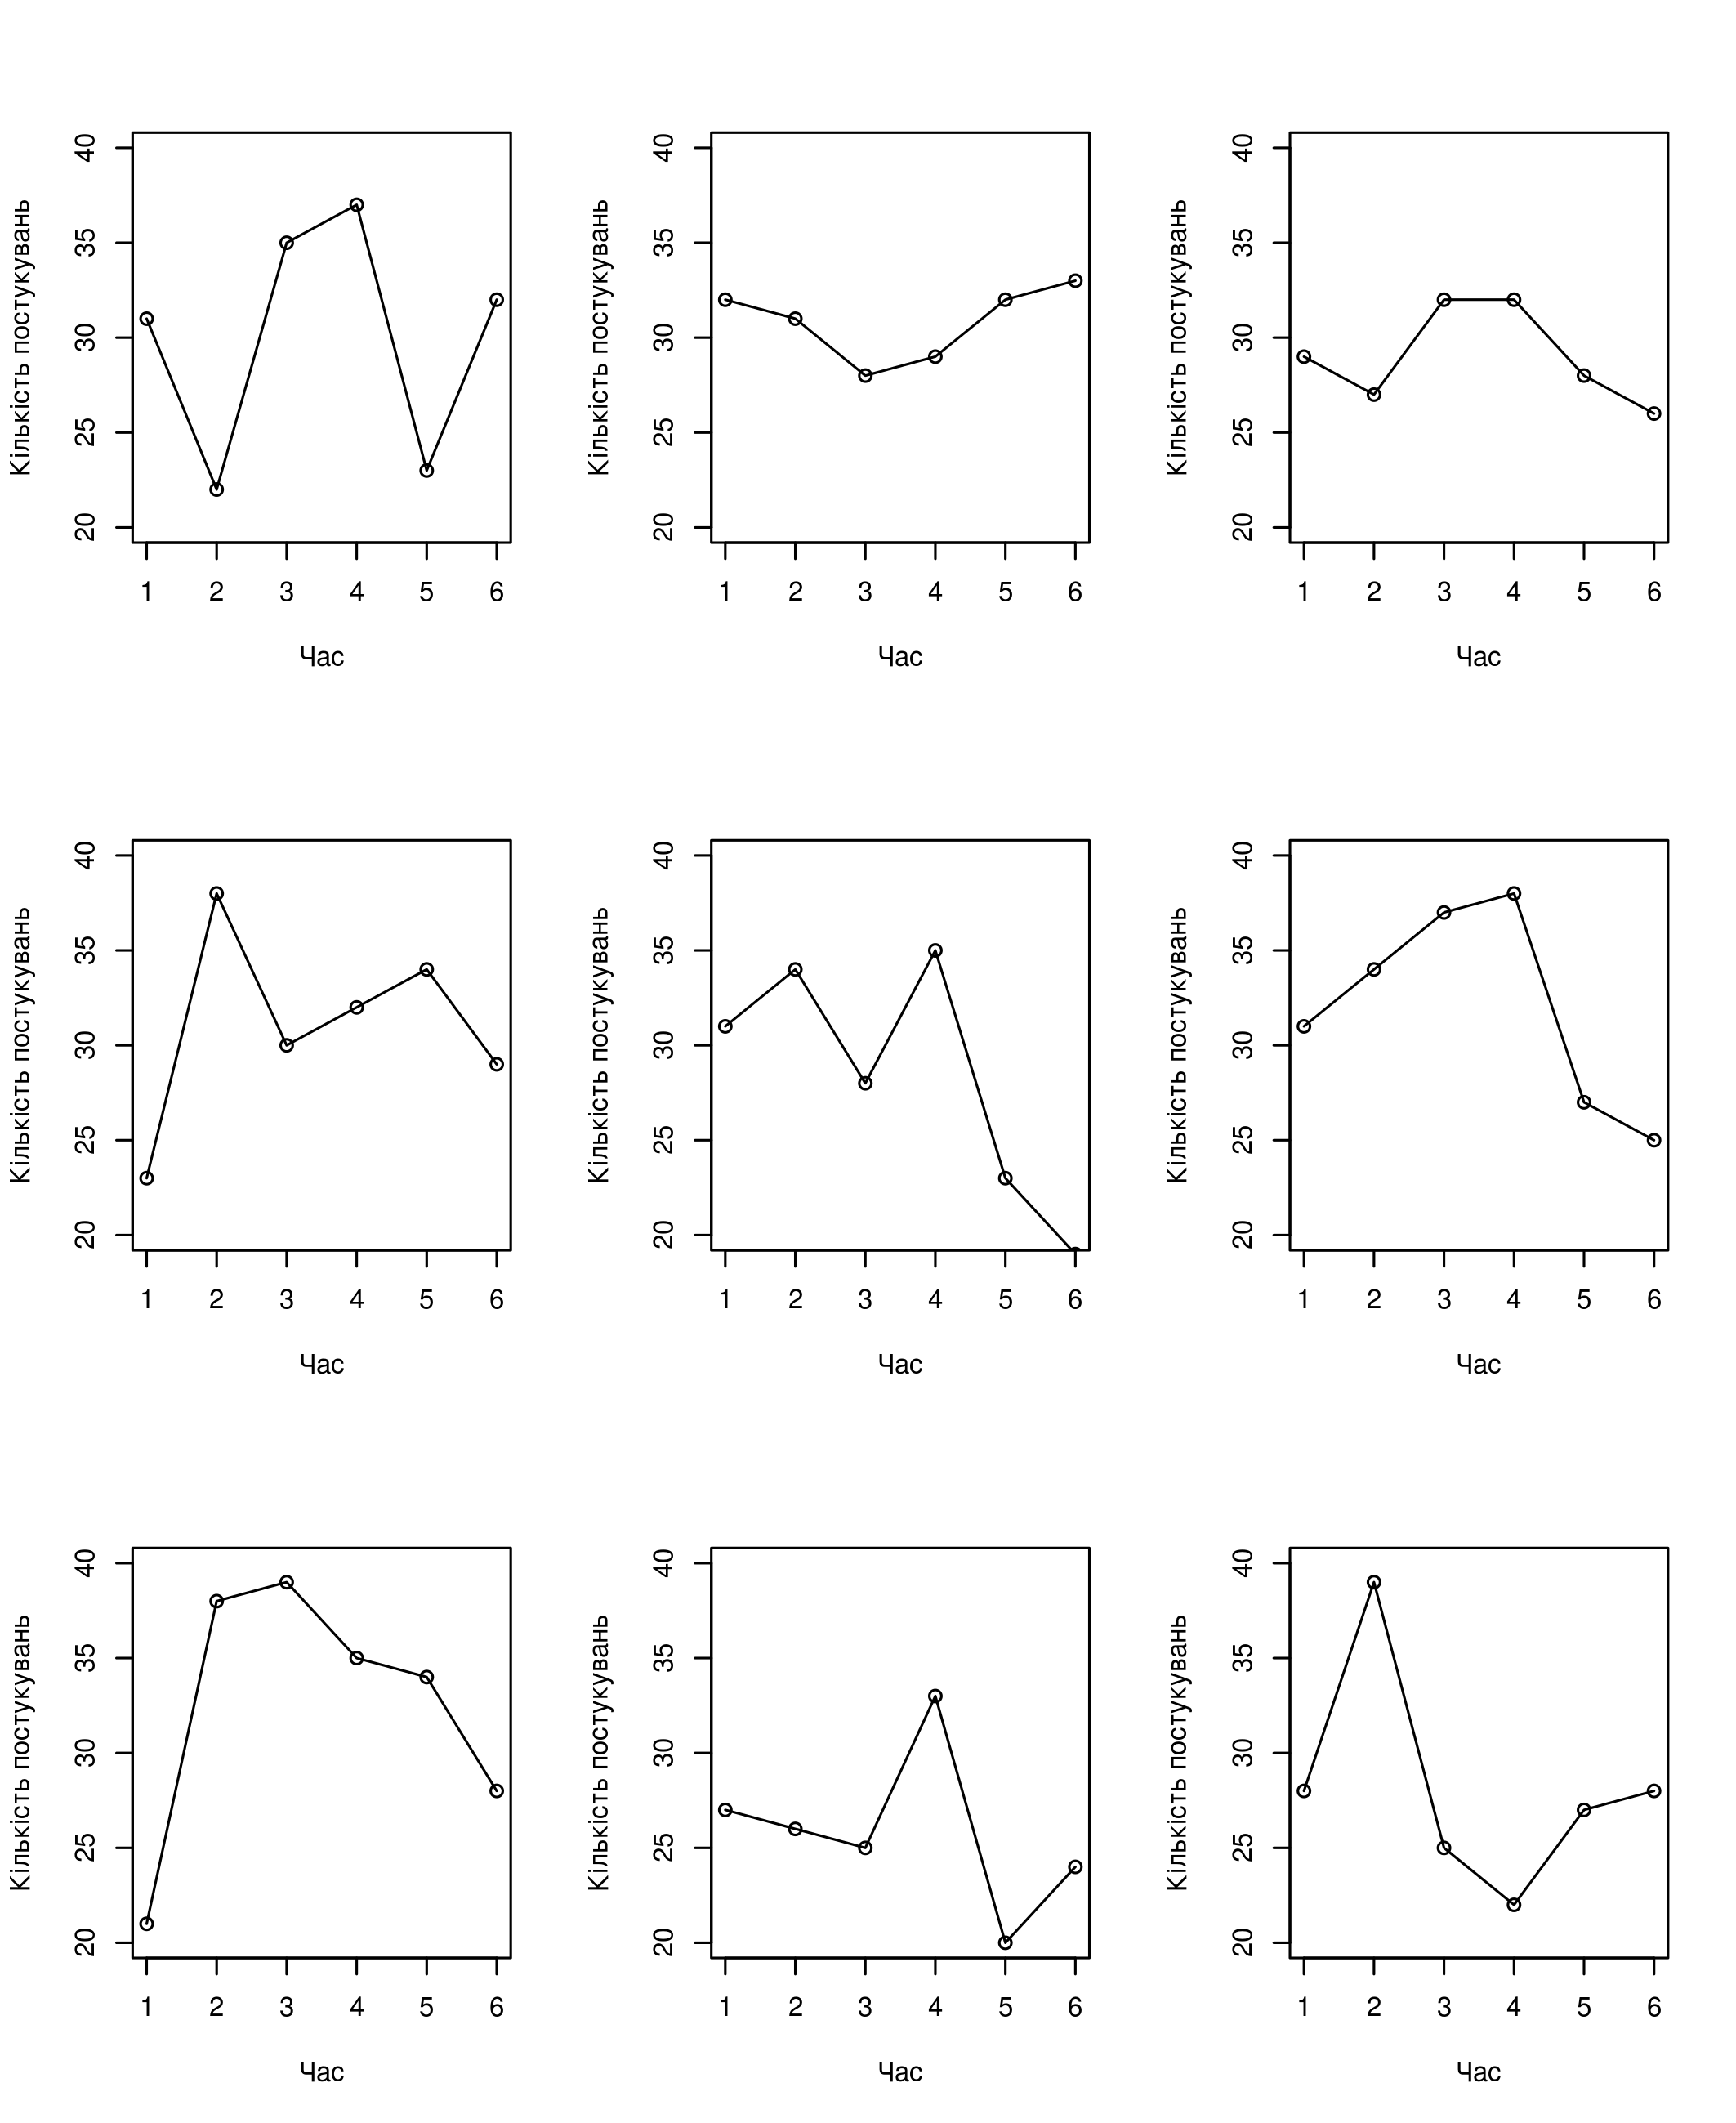
\includegraphics[width=0.5\textwidth]{code/example}
  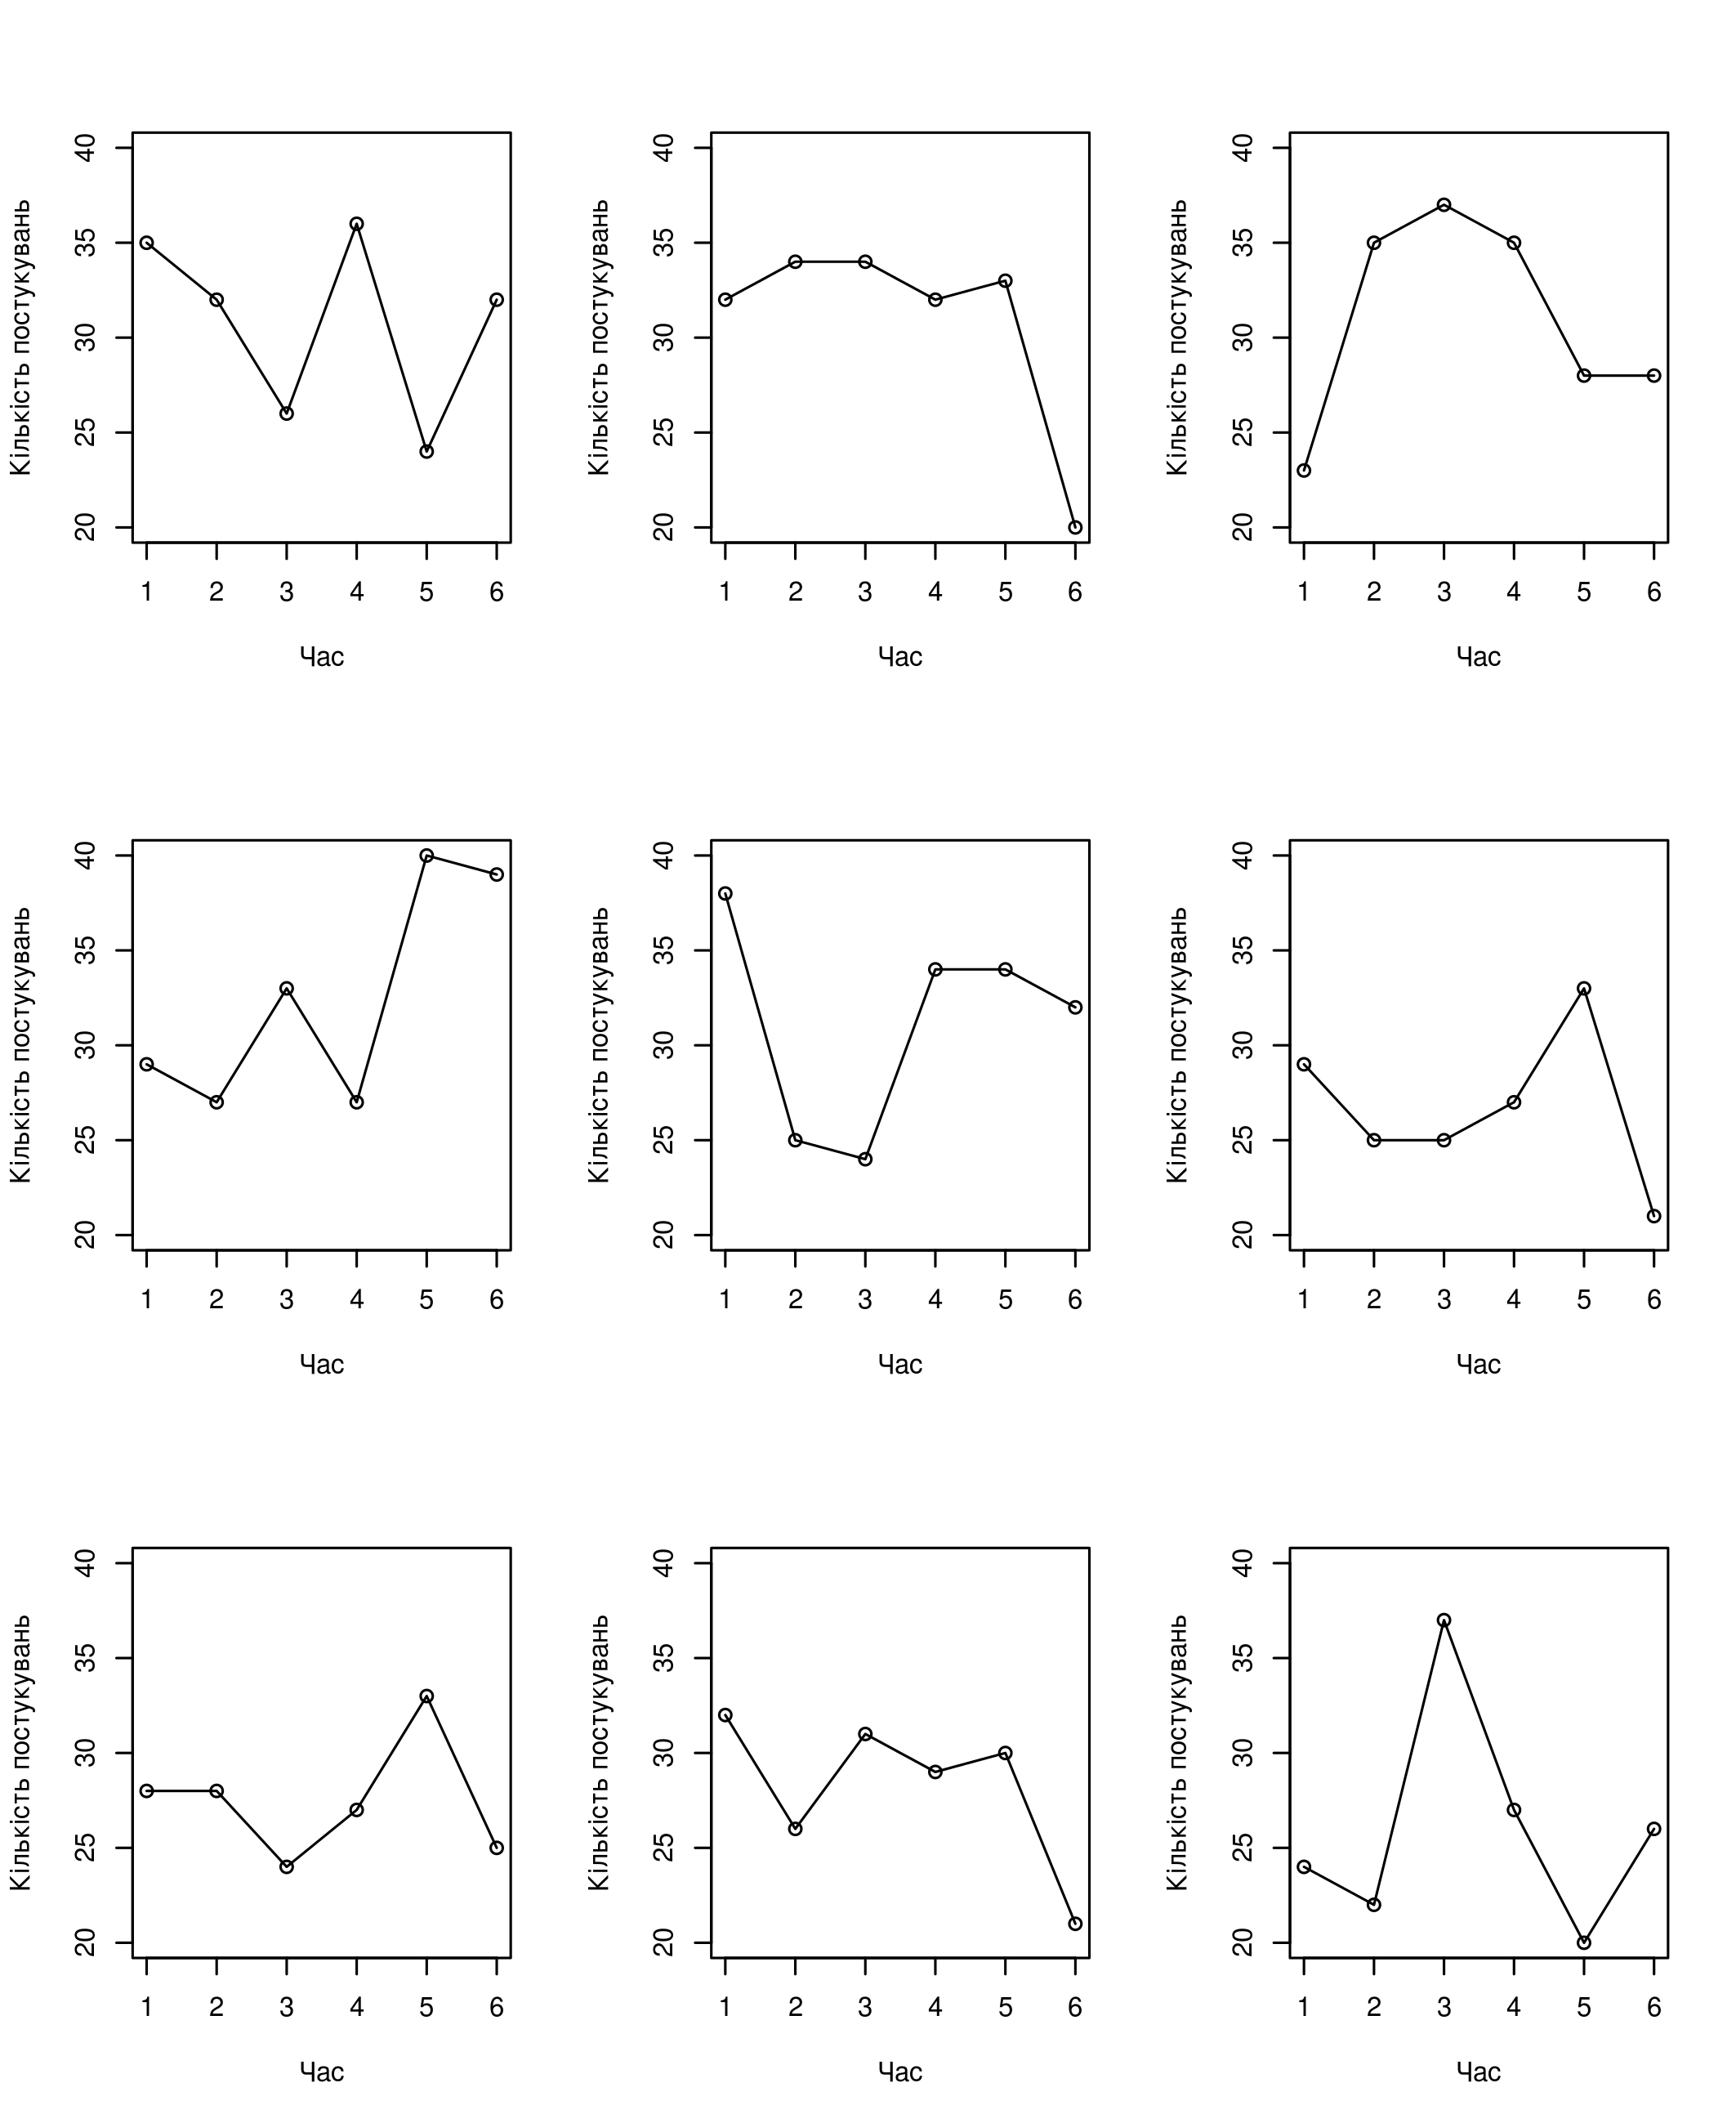
\includegraphics[width=.95\textwidth]{code/example_2.png}
  \caption{Приклад моделювання}
  \label{fig:tapping:poisson}
\end{figure}

\subsubsection{Квадратична апроксимація}

Види результуючих ламаних (опукла, ввігнута, рівна, спадна) можна представити
квадратичними функціями часу вигляду
\begin{equation*}
  y\left( t \right) = a \cdot t^2 + b \cdot t + c
\end{equation*}
Якщо знати напевно, що всі результати моделювання мають саме такий вигляд,
їх буде легко аналізувати.
Для цього скористаємось методом найменших квадратів для апроксимації результатів
моделювання.
На рис. \ref{fig:tapping:poisson:sqr} зображено реалізації послідовність
випадкових величин, що розподілені за законом Пуассона, та криві, що є
результатом апроксимації цих реалізацій.

\begin{figure}[h!]
  \centering
  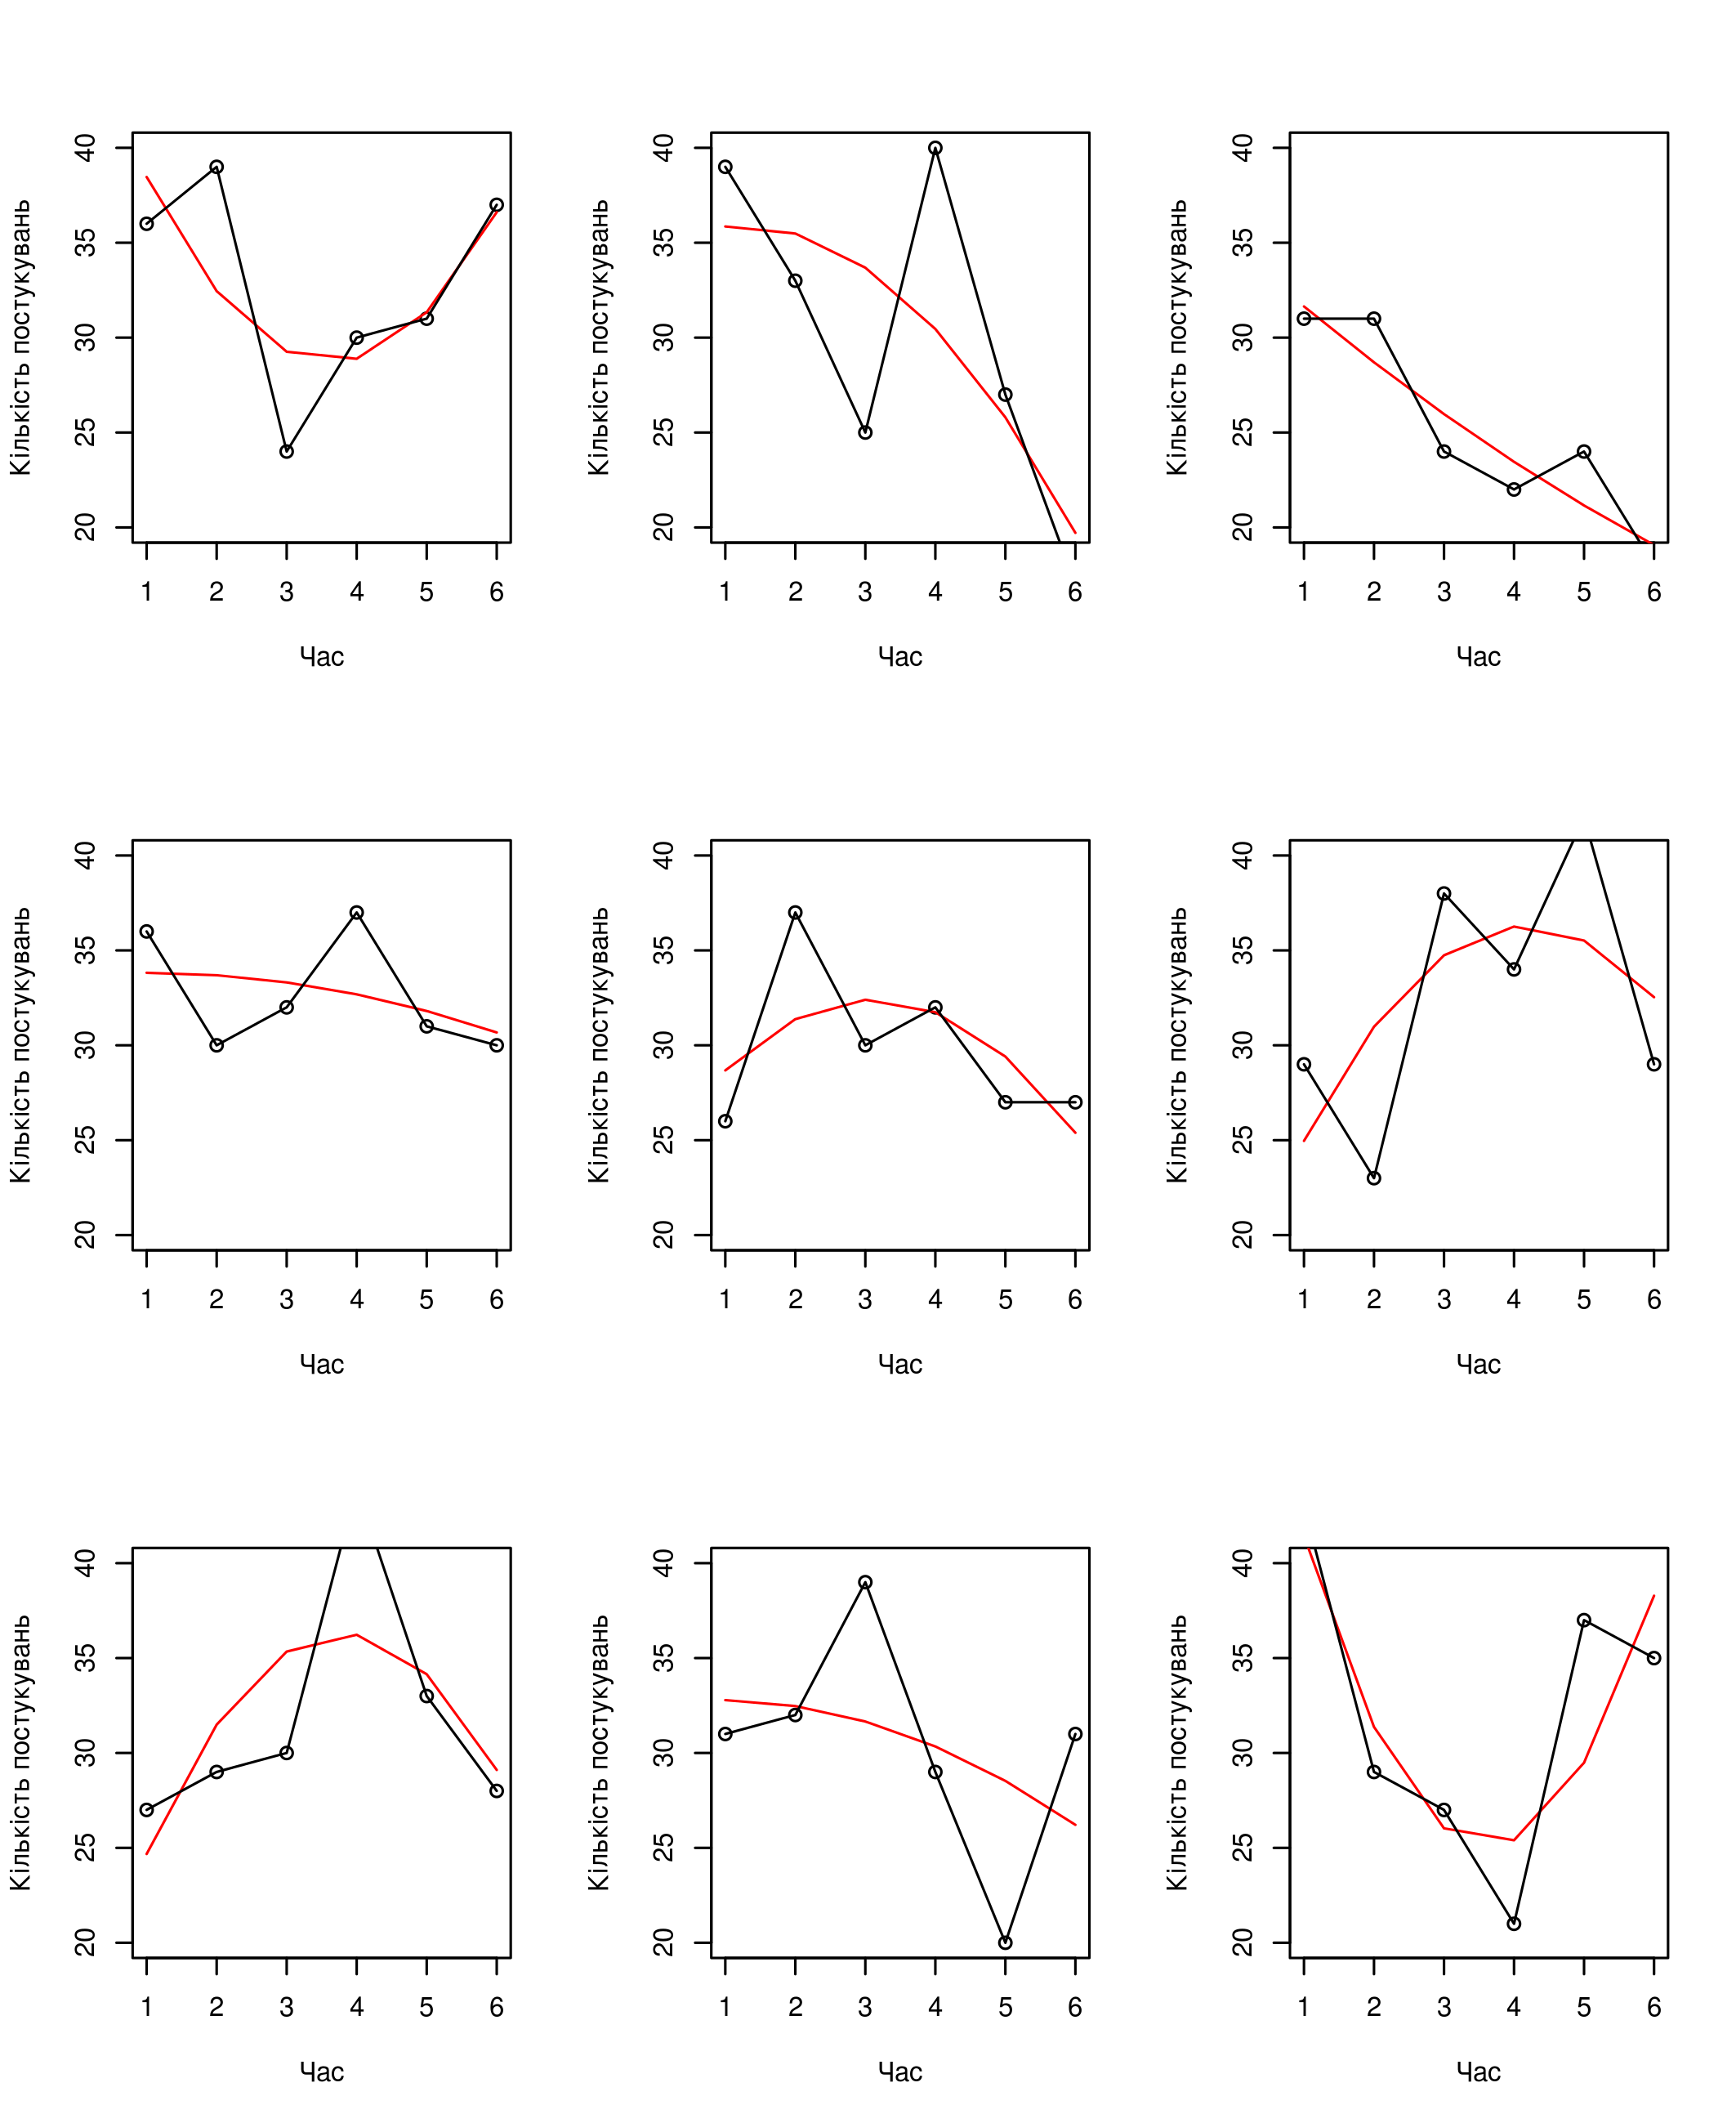
\includegraphics[width=.95\textwidth]{code/least_squares_approximation}
  \caption{Приклад моделювання з апроксимацією}
  \label{fig:tapping:poisson:sqr}
\end{figure}

Проаналізуємо ввігнуту параболу: $a > 0$.
Значення опуклої ламаної в кінцевій точці не може бути більшим,
ніж в початковій
\begin{equation*}
  a \cdot t_1^2 + b \cdot t_1 + c \ge a \cdot t_6^2 + b \cdot t_6 + c
\end{equation*}
Спростимо
\begin{equation*}
  a \cdot \left( t_1^2 - t_6^2 \right) + b \cdot \left( t_1 - t_6 \right) \ge 0
\end{equation*}
Поділимо обидві частини на $- a \cdot \left( t_1 - t_6 \right) > 0$
\begin{equation*}
  \frac{b}{-a} \ge t_1 + t_6
\end{equation*}

Опукла та проміжна ламані мають більш складні обмеження.
Перше обмеження: $a < 0$.
Також відомо, що опукла (проміжна) ламана досягає свого максимального значення не пізніше,
ніж в час $t_3$ ($t_2$), а під кінець спадає до початкового рівня або нижче.
Позначимо час, в який графік остаточно повинен почати спадати, через $t_f$.
Запишемо систему рівнянь
\begin{equation*}
  \begin{cases}
    \left. \frac{d\left( a \cdot t^2 + b \cdot t + c \right)}{dt}
      \right|_{t=t_{max}} &= 0 \\
    t_{max} &\le t_f \\
    a \cdot t_1^2 + b \cdot t_1 + c &\ge a \cdot t_6^2 + b \cdot t_6 + c
  \end{cases}
\end{equation*}
Розв’яжемо перше рівняння відносно $t_{max}$
\begin{equation*}
  \begin{cases}
    t_{max} &= \frac{-b}{2 \cdot a} \\
    t_{max} &\le t_f \\
    \frac{b}{-a} &\ge t_1 + t_6
  \end{cases}
\end{equation*}
Об’єднаємо систему в одне рівняння
\begin{equation*}
  t_1 + t_6 \le \frac{-b}{a} \le 2 \cdot t_f
\end{equation*}

Залишилося розглянути випадок прямого графіку.
Потрібно щоб значення функції змінилося не більше ніж на $\varepsilon = 1$.
У тому випадку, коли на проміжку $\left[ t_1, t_6 \right]$ отримана функція,
свого глобального екстремуму (максимуму або мінімуму) вона досягає на інтервалі
$\left( t_1, t_6 \right)$
\begin{equation*}
  0 \le t_1 < t_{g} = \frac{-b}{2 \cdot a} < t_6
\end{equation*}
У випадку опуклої (ввігнутої) параболи в точці $t_{g}$ досягається максимум
(мінімум) функції.

Запишемо нерівність, позначивши точку, де досягається локальний максимум,
через $t_{max}$, а точку локального мінімуму через $t_{min}$
\begin{equation*}
  - \varepsilon \le
  a \cdot \left( t_{max}^2 - t_{min}^2 \right)
    + b \cdot \left( t_{max} - t_{min} \right)
  \le \varepsilon
\end{equation*}
Запишемо нерівність через абсолютні значення та поділимо обидві частини на
$\left| t_{max} - t_{min} \right|$
\begin{equation}\label{eq:flat:abs}
  \left| a \cdot \left( t_{max} + t_{min} \right) + b \right|
  \le \frac{\varepsilon}{\left| t_{max} - t_{min} \right|}
\end{equation}
Піднесемо обидві частини рівняння до квадрату та перенесемо все вліво
\begin{equation*}
  b^2 + b \cdot 2 \cdot a \cdot \left( t_{max} + t_{min} \right)
    + a^2 \cdot \left( t_{max} + t_{min} \right)^2
    - \frac{\varepsilon^2}{\left( t_{max} - t_{min} \right)^2}
  \le 0
\end{equation*}
Розв’язок відносно $b$ має вигляд
\begin{equation*}
  -a \cdot \left( t_{max} + t_{min} \right) - \frac{\varepsilon}{t_{max} - t_{min}}
  \le b
  \le -a \cdot \left( t_{max} + t_{min} \right) + \frac{\varepsilon}{t_{max} - t_{min}}
\end{equation*}
Повернемося до рівняння \eqref{eq:flat:abs}.
Одна з точок $t_{max}$ і $t_{min}$ має значення $t_g$, а інша --- точка
локального екстремуму на кінці часового проміжку, що розглядається,
яку позначимо через $t_l$ ($t_1$ або $t_6$).
Відомо, що $t_{g} = \frac{-b}{2 \cdot a}$.
Введемо це значення в рівняння \eqref{eq:flat:abs}
\begin{equation*}
  \left| a \cdot \left( t_g + t_l \right) + b \right|
  \le \frac{\varepsilon}{\left| t_l - t_g \right|}
\end{equation*}
\begin{equation*}
  \left| a \cdot t_l + \frac{b}{2} \right|
  \le \frac{\varepsilon}{\left| t_l + \frac{b}{2 \cdot a} \right|}
\end{equation*}
Помножимо обидві частини на $\left| a \cdot t_l + \frac{b}{2} \right|$
\begin{equation*}
  \left( t_l + \frac{b}{2} \right)^2
  \le \left| a \right| \cdot \varepsilon
\end{equation*}
Випишемо отримане квадратне рівняння
\begin{equation*}
  b^2 + b \cdot 4 \cdot t_l + 4 \cdot t_l^2
    - 4 \cdot \left| a \right| \cdot \varepsilon
  \le 0
\end{equation*}
Після розв’язання нерівності отримаємо обмеження для $b$
\begin{equation*}
  -2 \cdot t_l - 2 \sqrt{\left| a \right| \cdot \varepsilon}
  \le b
  \le -2 \cdot t_l + 2 \sqrt{\left| a \right| \cdot \varepsilon}, \qquad
  t_1 < \frac{-b}{2 \cdot a} < t_6
\end{equation*}
